\chapter{Background}\label{chapter:background}

This chapter introduces relevant background information on
best practice guidelines (\BPG{}) and guidelines-based clinical decision support
systems (\CDSS{}).
In \autoref{sec:bpg-background}, we utilize a real-world \BPG{}
to explain the motivation behind codifying treatment
in the form of clinical guidelines. We also briefly discuss
common characteristics of such guidelines that enable medical knowledge
to be represented efficiently and accurately.

\BPGs{} are usually published by hospitals,
research institutions and medical associations with the aim to improve quality of care by
\begin{enumerate*}[label=(\alph*)]
  \item reducing medical errors due to preventable causes,
  \item standardizing knowledge from latest evidence-based research, and,
  \item enabling access to aforementioned knowledge at medical establishments
  that lack resources to conduct research.
\end{enumerate*}

While in theory, following \BPGs{} should improve clinical outcomes,
their effectiveness in practice is dictated by whether healthcare practitioners
follow them or not. In \autoref{sec:cdss-background}, we present
challenges that practitioners encounter in following \BPGs{}. We then argue
that non-conformance results in worse patient outcomes.
Next, we show how computerized systems that utilize data from available
heterogeneous sources such as electronic health records and sensors for
patient parameters can improve patient outcomes by addressing challenges
to following \BPGs{} encountered by practitioners.

\section{Clinical Best Practice Guidelines}\label{sec:bpg-background}

Clinical best practice guidelines are evidence-based statements
published by hospital and medical associations that codify recommended
interventions for various clinical scenarios \cite{field1990clinical}.
It has been recognized that, if implemented correctly, \BPGs{} have the potential to:

\begin{enumerate}
  \item Reduce unwarranted variations in clinical practice.
  \item Improve healthcare safety and quality.
  \item Enhance translation of research into practice.
  \item Reduce healthcare costs.
  \item Enable development of performance measures for diseases
    \cite{GuerraInjury23, BusseWHO19}.
\end{enumerate}

Guidelines in the form of statements and recommendations
were first introduced in the 1970s,
and were mostly based on expert opinion
In the 1980s and the early part of 1990,
a significant increase in evidence from proliferation of randomized controlled
trails occured. This co-incided with the introduction
of computers at medical instutions that enabled available evidence
to be quickly accessed to aid decision making \cite{GuyattAMA92,SackettJPH95}.
These developments facilitated a shift towards more rigorous
development of \BPGs{}, where evidence was prioritized over expert opinion
\cite{GuerraInjury23}.

To be able to administer optimum care, practitioners must take into
account evidence from ongoing research to guide treatment. This
can be particularly challenging, as available evidence can evolve rapidly.
\BPGs{} enable findings from latest research to be quickly translate in
practice. Well designed \BPGs{} are usually developed and published by trusted medical
establishments (such as medical associations and research institutions)
that base recommendations on best available evidence \cite{GuerraInjury23}.
As the body of evidence increases over time through research,
\BPGs{} must be updated accordingly to reflect latest findings.

\begin{figure}[t]
  \centering
  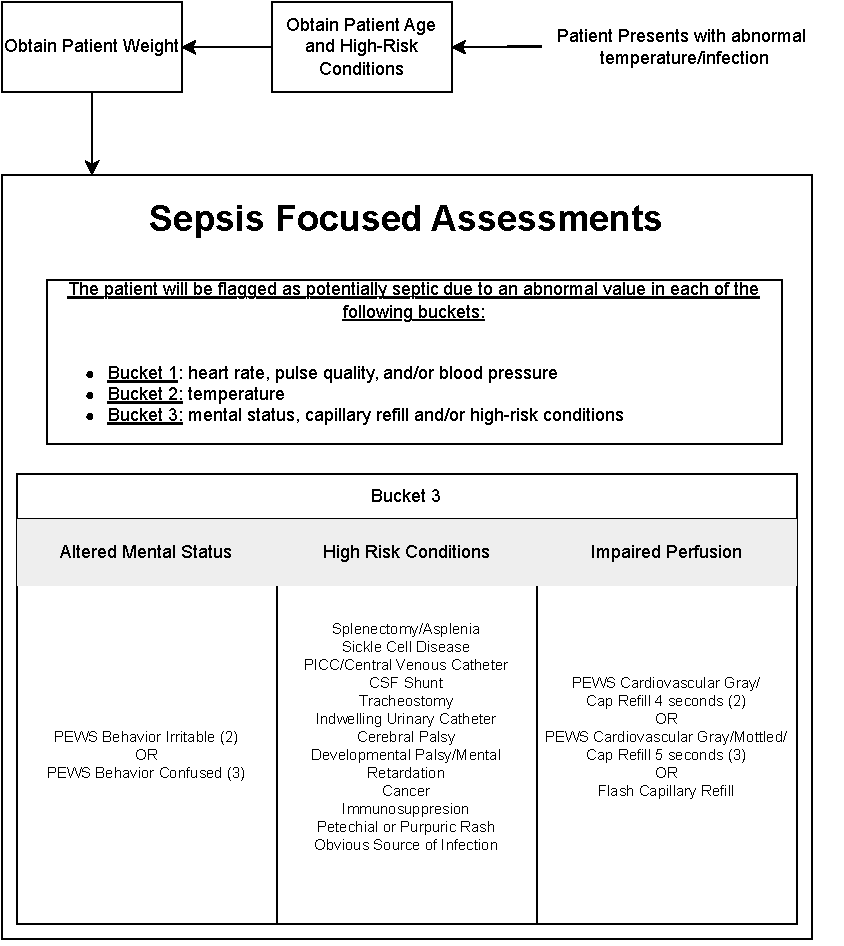
\includegraphics[width=0.5\textwidth]{sepsis-screening-osf}
  %\includegraphics[width=0.5\textwidth]{screening-vitals}
  \caption{Pediatric sepsis screening \BPG{}}\label{fig:sepsis-screening}
\end{figure}

To illustrate characteristics of \BPGs{}, we briefly go over a \BPG{}
for managing sepsis in pediatric cases used at OSF St. Francis Medical Center
in Peoria, Illinois -- a major pediatric hospital in the United States. Note
that for brevity, we refer to said hospital simply as OSF in the remainder of
this section.
Sepsis is life-threatening condition caused by the body's extreme response to
an infection \cite{RhodesICM17}, and is
a major cause of morbidity and mortality in children \cite{Eisenberg2021JP}.
Adverse outcomes can, however, be mitigated through timely
identification and prompt treatment with antibiotics and
intravenous (IV) fluids \cite{Weiss2014CCM,Evans2018JAMA}.
\BPGs{} for screening and management of sepsis in pediatric Emergency
Departments (EDs) have shown effectiveness in screening and management of sepsis \cite{Eisenberg2021JP},
leading to their adoption in many pediatric EDs \cite{Balamuth2017EM,Sepanski2014FP}.

In \autoref{fig:sepsis-screening}, we present a simplified version of
the screening section of OSF's sepsis mangement guideline.
In essence, when a patient arrives at the
\ED{} with a fever or an infection, the \HCP{} is supposed to obtain
\begin{enumerate*}[label=(\alph*)]
  \item the patient's age,
  \item any conditions, such as cancer, immunosuppresssion, etc,
    that increase likelihood of sepsis, and
  \item the patient's vital signs, such as heart rate, systolic blood
    pressure, respiratory rate, etc.
\end{enumerate*}

This information is then used to check for abnormalities
in clusters of linked information, called \say{buckets}. For instance, if
the patient's heart rate is abnormal, then \say{bucket 1} is said to
have an abnormal value.
Checking for such abnormalities often involves the use of tables, such as
\autoref{table:vital-signs} that contains normal ranges indexed by
\emph{age}.
%\footnote{For brevity, we omit some age ranges and vital signs from table
%\ref{table:vital-signs}}.
If the patient has at least one abnormal value in every \say{bucket},
then he/she is flagged as potentially septic.

The \BPG{}-recommended treatment for
sepsis involves multiple concurrent workflows, such as
screening for septic shock, fluid resuscitation, and administering antibiotics.
In \autoref{fig:fluid-therapy}, we provide
a version of the fluid resuscitation guideline used
at OSF. Briefly, if the patient is flagged as potentially septic, the guideline suggests
\begin{enumerate*}[label=(\roman*)]
  \item obtaining any fluid-overload risks,
  \item administering normal saline (typically over a period of 15 minutes),
    where the dosage is dictated by risks determined in previous step,
  \item assessing signs of fluid-overload,
  \item evaluating patient responsiveness to normal saline upon completion of
    the administering process, and,
  \item determining whether another fluid bolus should be administered based on
    information from previous steps.
\end{enumerate*}
\begin{figure}[h]
  \centering
  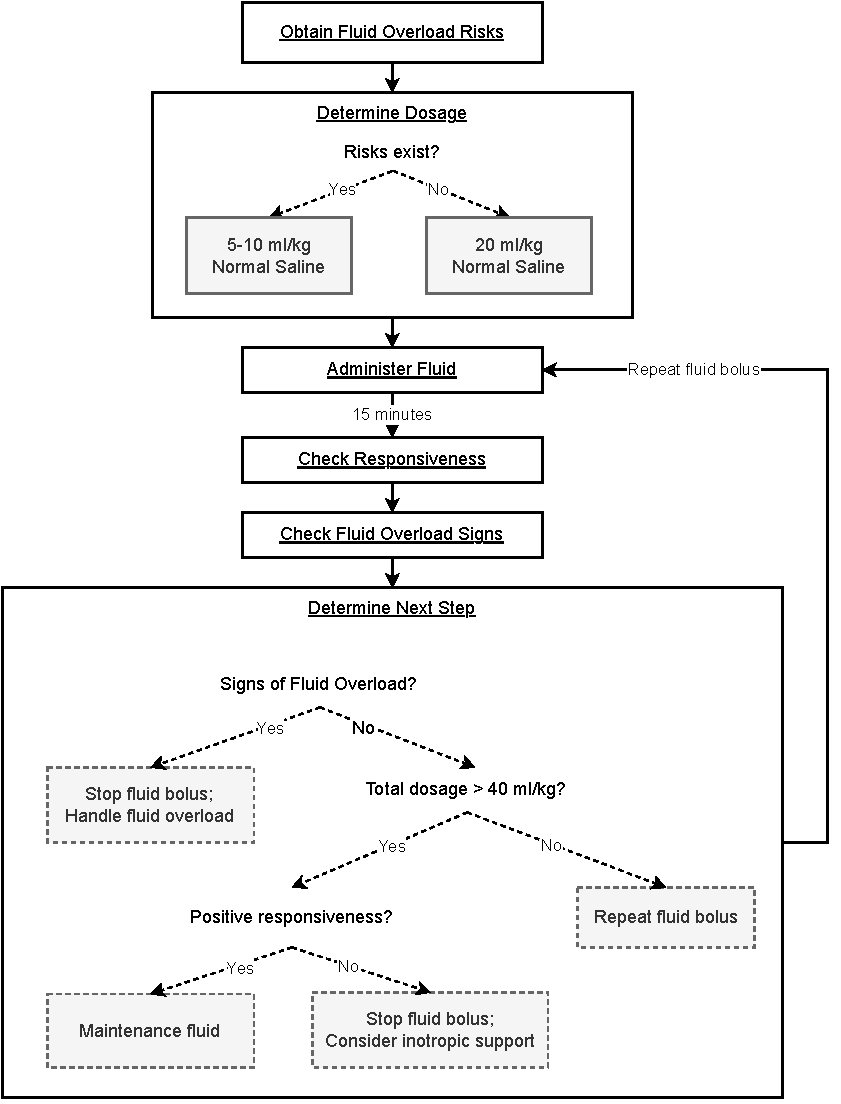
\includegraphics[scale=0.5]{FluidWorkflow-fmcad.pdf}
  \caption{Fluid Resuscitation Guideline}\label{fig:fluid-therapy}
\end{figure}

  \begin{table}
    \centering
    \begin{tabular}{ | c || c | c | c | }
      \hline
      \textbf{Age}            & \textbf{Heart Rate}   & \textbf{Systolic BP} & \textbf{Temp}  \\
      \hline
      $0d - 1m$               & $>205$                & $<60$                & $<36 \text{ or } >38$ \\
      \hline
      $\geq 1m - 3m$          & $>205$                & $<70$                & $<36 \text{ or } >38$ \\
      \hline
      $\geq 3m - 1y$          & $>190$                & $<70$                & $<36 \text{ or } >38.5$ \\
      \hline
      $\dots$                 & $\dots$               & $\dots$              & $\dots$ \\
      \hline
      $\geq 13y$              & $>100$                & $<90$                & $<36 \text{ or } >38.5$ \\
      \hline
    \end{tabular}
    \caption{Vital Signs Chart}\label{table:vital-signs}
  \end{table}

This real-world \BPG{} exhibits characteristics common
across many \BPGs{}. Specifically \BPGs{} typically:
\begin{itemize}
  \item Involve \stress{concurrent} workflows, such as administering drugs,
    monitoring vitals, performing treatment, etc. There may also be
    inter-workflow interactions. For instance, a diagnosis of sepsis during the
    screening may require modifications to an ongoing course antibitiotics.
  \item Often specified in a \stress{flowchart-like}
    notation. See \cite{AHAFlowcharts} and \cite{CancerCareFlowcharts} for other flowchart-based \BPGs{} for management of \emph{cardiac arrest}, and
    screening, risk-reduction, treatment and survivorship in
    cancer care respectively.
  \item Require communication between \stress{heterogeneous agents} such as
     monitors and Electronic Health Records (EHRs).
  \item Often use \stress{tables} indexed by parameters such as age, weight,
    etc to present normal/abnormal ranges for measurements, or recommended dosages for drugs.
\end{itemize}

Note that the aforementioned characteristics are \emph{not} specific
to one guideline. According to a review paper on \CIGs{} \cite{ClerqAIM03},
such \DSLs{} should additionally
\begin{enumerate*}[label=(\alph*)]
  \item be formally defined, i.e, have a formal syntax and semantics, and
  \item have an execution engine to provide decision support.
\end{enumerate*}

\section{Clinical Decision Support Systems}\label{sec:cdss-background}

\BPGs{} are developed with the intention of improving patient outcomes
by reducing preventable medical errors. But, such guidelines can only be
effective if they are followed in practice, which can be challenging.
 For instance, consider the Advanced Cardiac Life Support (ACLS):
a \BPG{} published by the American Heart Association (AHA) for management
of a life-threatening condition called in-hospital cardiac arrest
\cite{AHAGuidelineAdult, AHAGuidelinePed}. Studies suggest that management
of IHCA in 30\% of adult, and 17\% of pediatric cases deviates from the
AHA-prescribed \BPG{}, resulting in worse patient outcomes \cite{Ornato2012DeviationAdult,Wolfe2020DeviationPediatric,
Crowley2020DeviationAdult,Honarmand2018Adherence,Mcevoy2014Adherence}.

The benefits of \BPGs{} have resulted in them being widely adopted
in daily practice \cite{WoolfBMJ99}. However, \BPG{} adoption in
clinical settings has several challenges. \BPGs{} are complex documents,
which may also contain some vagueness.
Exact meaning of terms is not always defined and recommended
actions may not be clearly articulated. The long and cumbersome
nature of \BPGs{} may make them difficult to effectively apply
in regular practice. Additionally, such \BPGs{} need to be
periodically updated to take into account latest evidence, and
adapted according to local needs of the setting they're utilized
in \cite{DeClerqSHTI08}.

To mitigate aforementioned issues, systems that utilize available
patient data to assess patient state and issue guideline-based
decision support to practiioners can be utilized \cite{DeClerqSHTI08}.
Such computerized clinical decision support systems (\CDSSs{}) codify
medical knowledge in \BPGs{} and provide practitioners with
situation-specific advice that \say{guides} them towards adherence
to the underlying \BPG{}.
Well implemented \CDSSs{} have been shown to improve
\BPG{}-adherence \cite{GargJAMA06,KawamotoBMJ05}, and reduce
\PMEs{} based on evidence from multi-center clinical trials \cite{BenettJAMIA16,SahotaJIS11}.

\subsection{\CDSS{} Example}\label{sec:cdss-example}

In \autoref{sec:bpg-background}, we presented a real-world
\BPG{} for screening and management of sepsis in pediatric cases.
To illustrate how a \CDSSs{} can enable better \BPG{} adherence,
we utilize an example \CDSS{} that codifies the sepsis management \BPG{}
to administer decision support.

In \autoref{fig:sepsis-tool}, we show an overview
of a \CDSS{} for sepsis management.
The \CDSS{} is intended to work as tablet at
the patient's beside in a hospital's emergency department (ED).
\autoref{fig:sepsis-tool-main} depicts main screen that the practitioner sees on the tablet.
The main screen consists of four panes (labeled and color coded for illustration
purposes). Pane 1 shows a grid with the patient's vitals pulled
from a combination of the patient's records, sensor measurements and
assessments made by practitioner through prompts that appear on the screen.
Red and green depict abnormality and normality respectively, while gray
indicates missing measurements, which are assumed to be normal. As more
measurements become available, corresponding boxes in the grid are updated
to reflect their status. The two boxes in the top left corner depict whether
the patient is suspected to have sepsis, and be in septic shock. The \CDSS{}
continually monitors these vitals to determine whether they satisfy the criteria
for sepsis or septic shock specified in the hospitals guideline, where the
guideline itself is a $\MediK{}$ program that the practitioners can view and
comprehend. Pane 2 shows the tasks the practitioner is expected to perform
once sepsis is detected. As these tasks are supposed to be performed within an
hour (referred to as golden hour in sepsis treatment), the \CDSS{} tracks time
since the first task is started by clicking the corresponding check-mark.
For some complex tasks, such as fluid resuscitation and antibiotics
administration, an auxiliary window guides the practitioner through the task. The
example scenario shows a patient with concerning vitals despite having
given multiple fluid boluses, indicating septic shock -- a condition that
demands immediate attention. Thus, as specified in the guidelines, the system
recommends urgently administering antibiotics alongside fluids, by highlighting
the relevant tasks in yellow.
Pane 3 contains medications grouped by type, where clicking the
\say{GIVE} button corresponds to administering the drug.
Pane 4 leads to toggleable windows with
important information. For instance, clicking on \say{HAEMODYNAMICS LINE GRAPHS}
toggles the window in \autoref{fig:sepsis-graphs-view} depicting
the patient's vitals over time punctuated by points at which
drugs were administered.

%\begin{figure}[t]
%  \centering
%  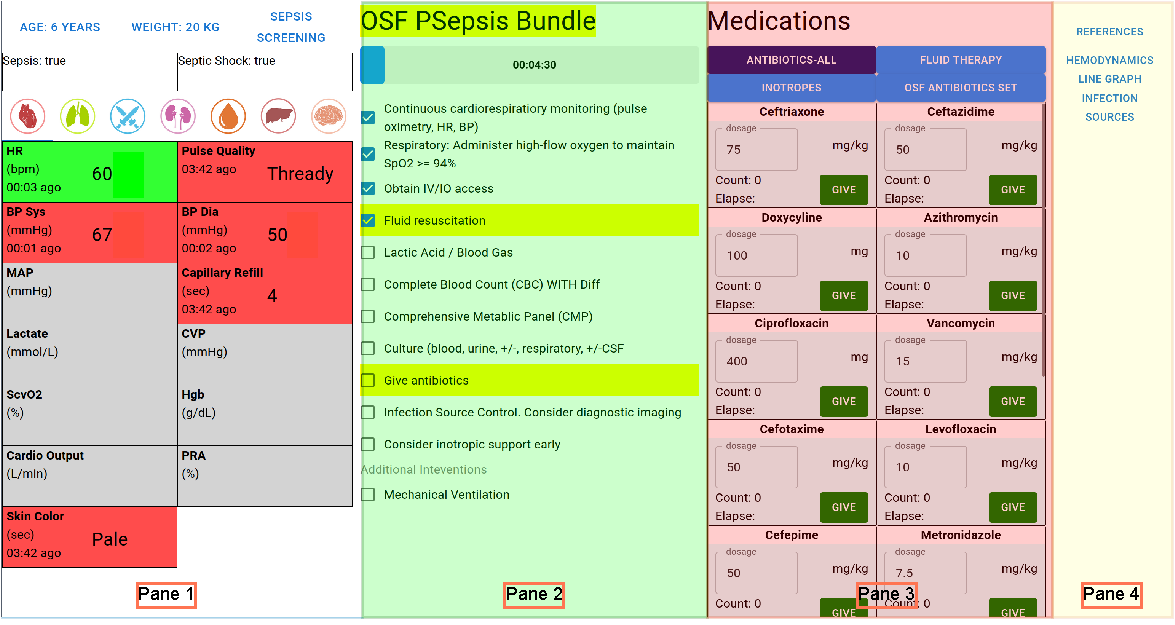
\includegraphics[width=0.7\textwidth]{sepsis-tool-main}
%  \caption{Sepsis Tool Main Screen}\label{fig:sepsis-tool-main}
%\end{figure}
%
%\begin{subfigure}[b]
%  \centering
%  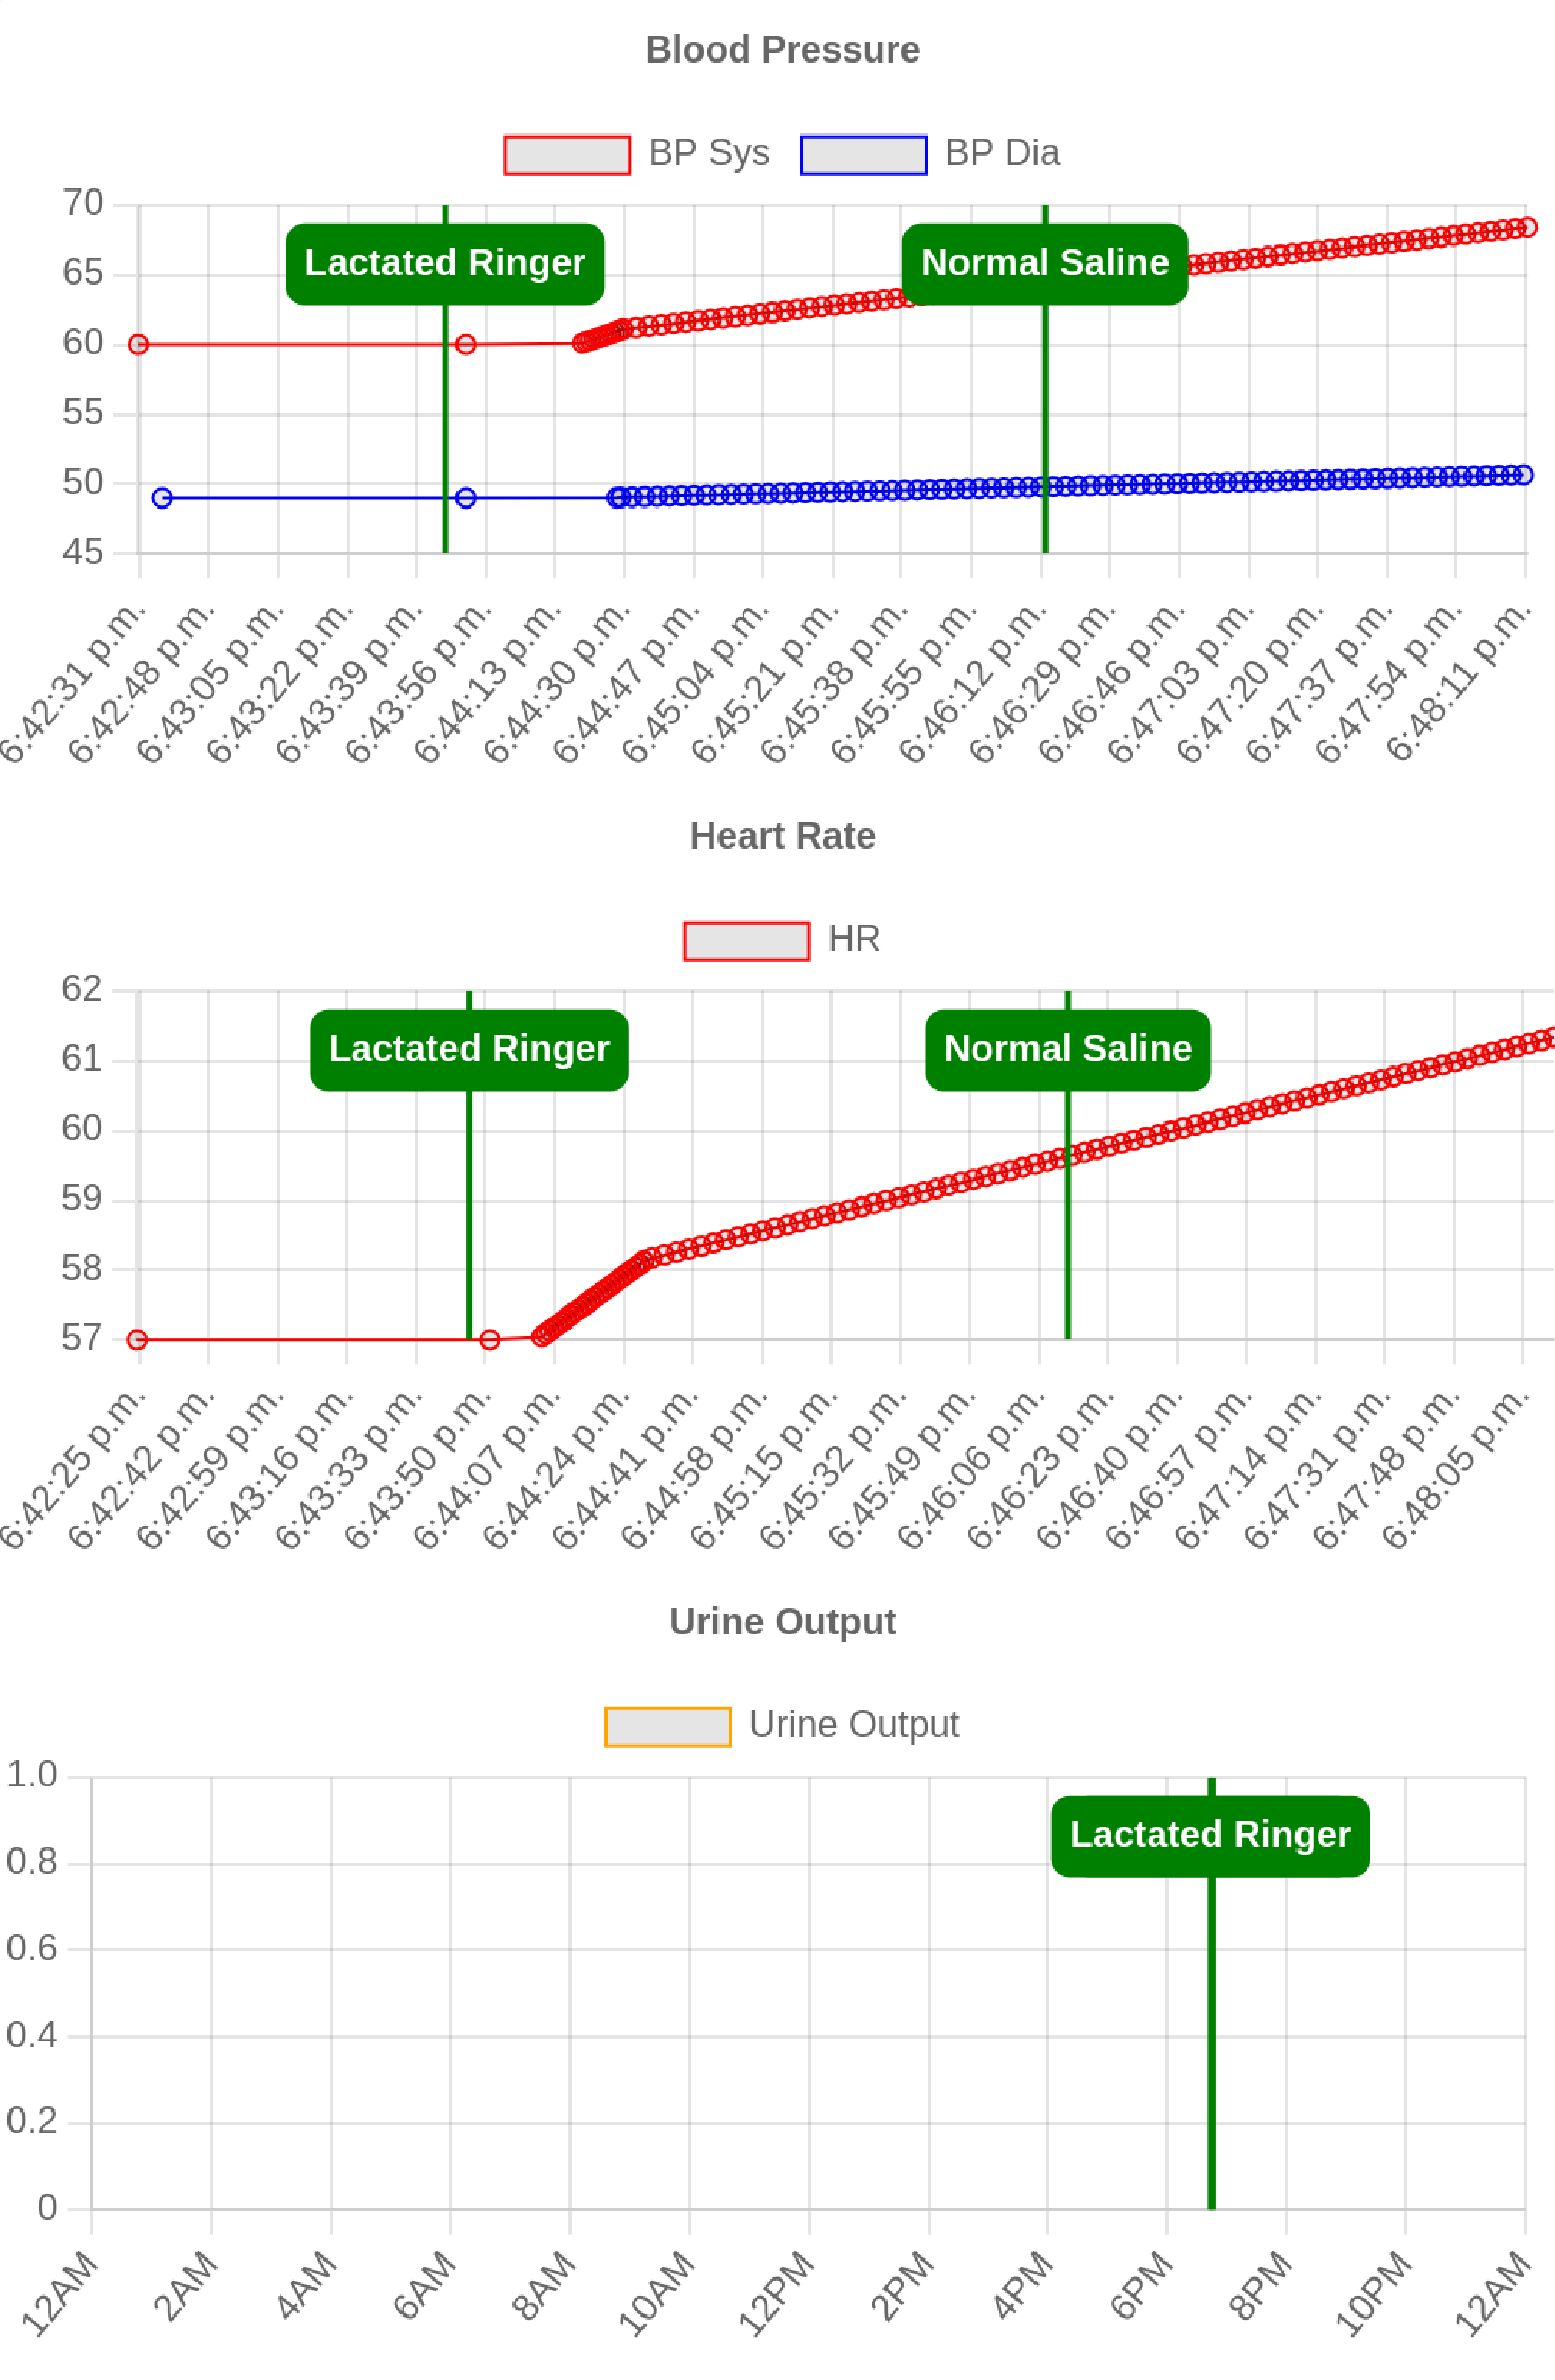
\includegraphics[width=0.5\textwidth]{sepsis-graphs}
%  \subcaption{Patient Vitals vs Time}\label{fig:sepsis-graphs-view}
%\end{subfigure}

\begin{figure*}[t!]
  \begin{subfigure}[t]{0.69\textwidth}
    \centering
    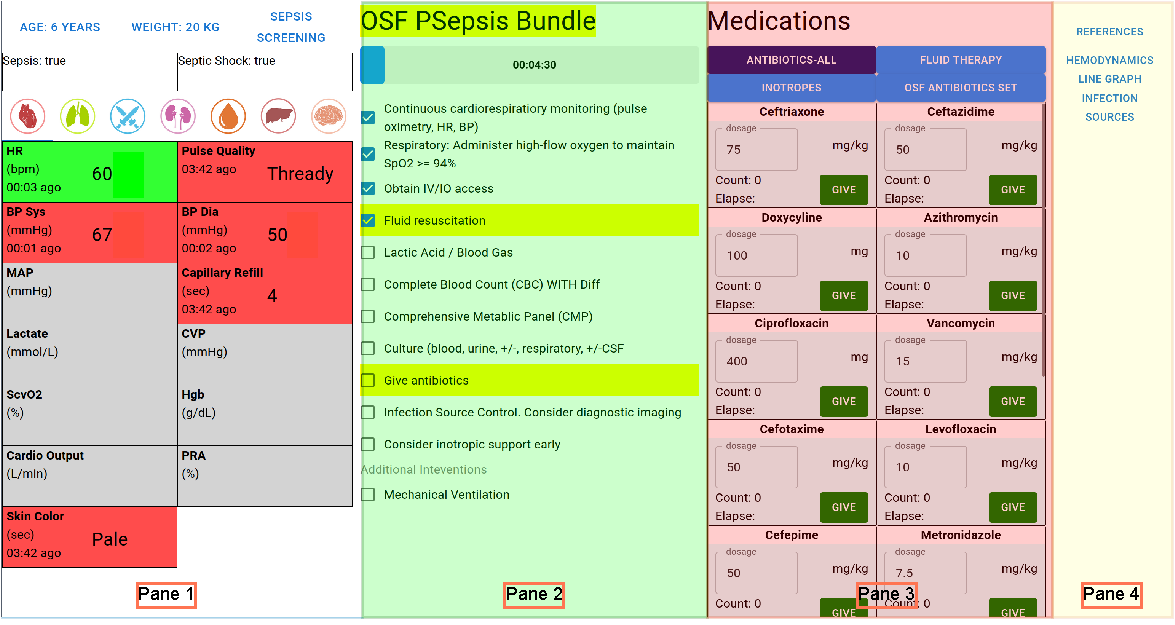
\includegraphics[height=2.5in]{sepsis-tool-main}
    \subcaption{Main Screen}\label{fig:sepsis-tool-main}
  \end{subfigure}
  \begin{subfigure}[t]{0.3\textwidth}
    \centering
    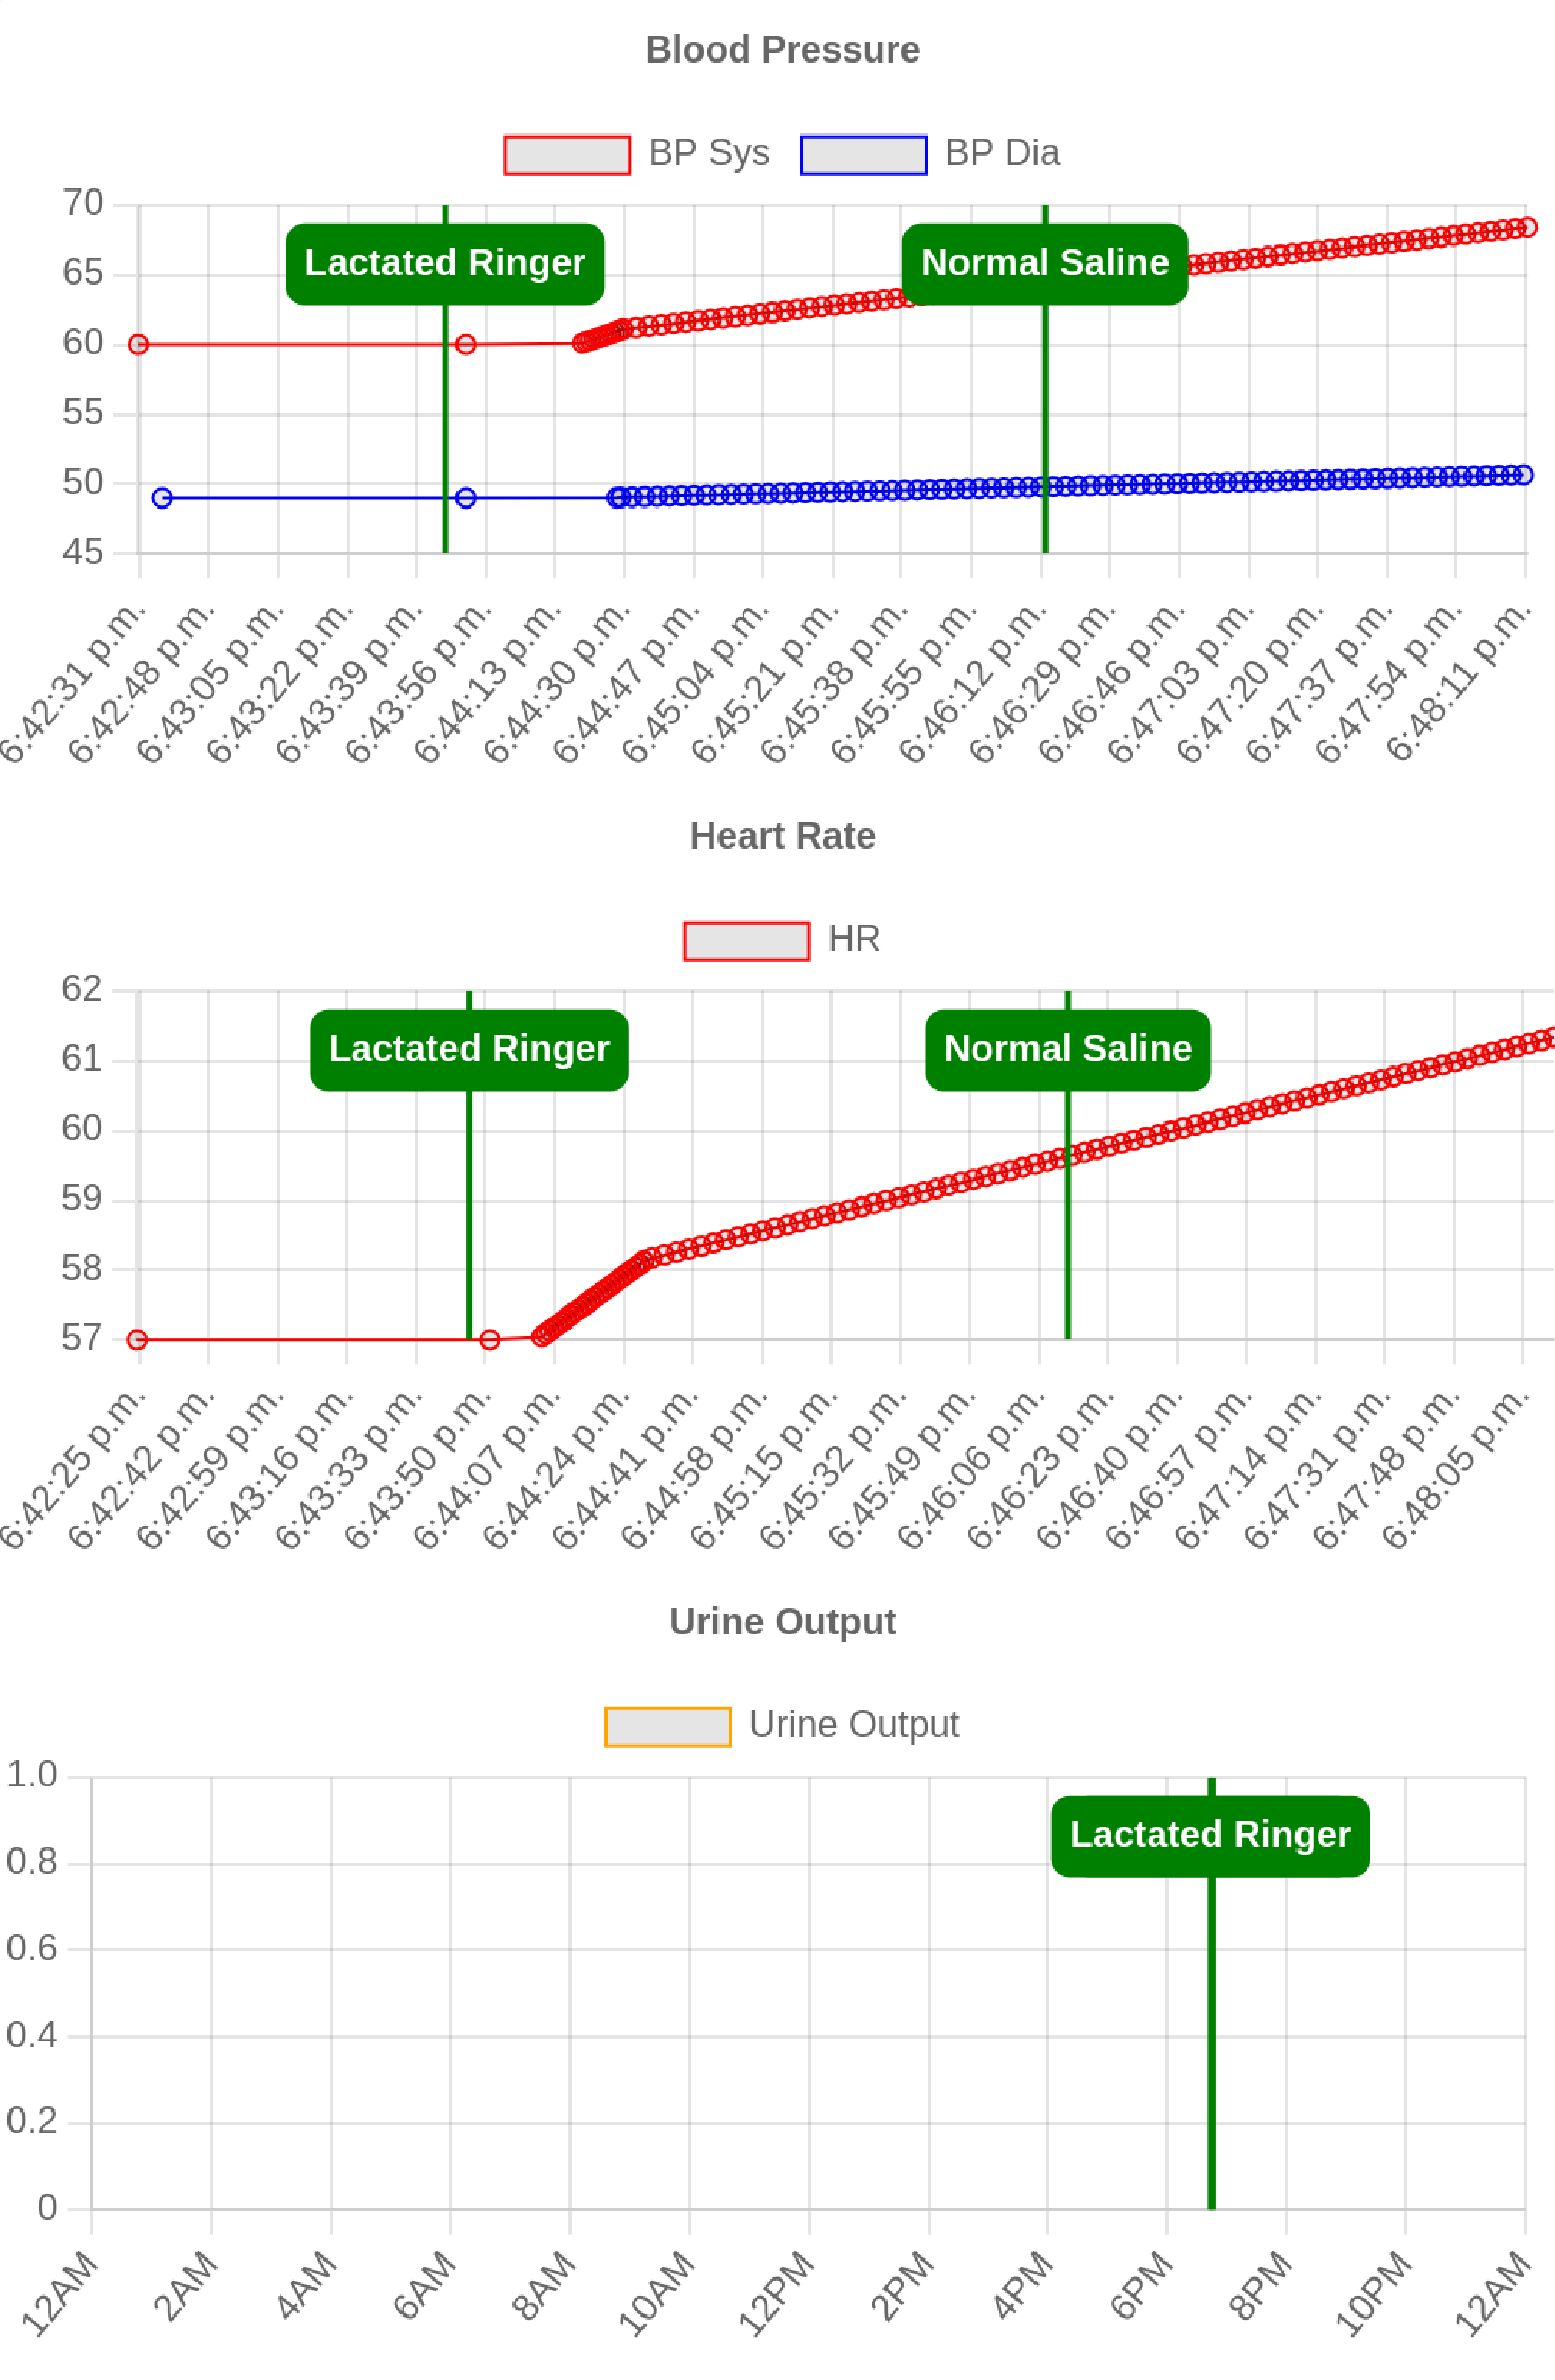
\includegraphics[height=2.5in]{sepsis-graphs}
    \subcaption{Patient Vitals vs Time}\label{fig:sepsis-graphs-view}
  \end{subfigure}
  \caption{$\MediK{}$-based Sepsis Management \CDSS{}}\label{fig:sepsis-tool}
\end{figure*}

\subsection{\CDSS{} Components}\label{sec:cdss-components}

\CDSSs{} were first introduced in the 1970s. Initial systems
didn't integrate well with existing patient care workflows, and
didn't find greater adoption outside academia. However,
wider adoption of electronic health records and digital systems for
patient parameters enabled better integration of \CDSSs{} with
workflows in everyday practice, enabling wider adoption.
Modern \CDSS{} can deliver recommendations
through a diverse spectrum of devices such
as systems at the patient bedsides, desktops or tablets carried by
practitioners and smartphones. This versatility
has further enhanced \CDSSs{} adoption \cite{SuttonNature20}.

\begin{figure}[t!]
  \centering
  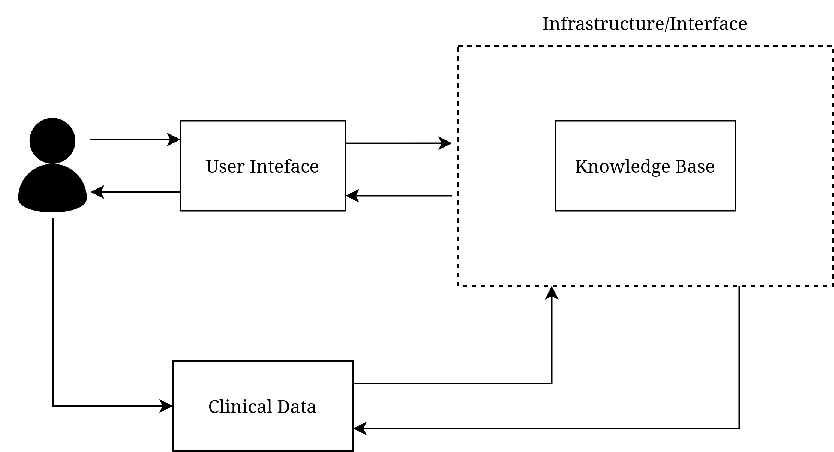
\includegraphics[width=0.75\textwidth]{cdss-architecture}
  \caption{\CDSS{} Components}\label{fig:cdss-architecture}
\end{figure}

In \autoref{fig:cdss-architecture}, we provide an overview
of the components of a typical \CDSS{}, and the underlying architecture.
A typical guidelines-based \CDSS{} conceptually consists of the
following components \cite{SuttonNature20}:

\paragraph{Knowledge Base:}

The knowledge base is the encoding of the underlying guideline in a
computable medium. Recall from \autoref{sec:bpg-background}
that \BPGs{} are typically developed experts in medicine and published
as textual documents. To develop a \CDSS{}, experts in medicine
collaborate with computer scientists or software developers to
develop requirements documentations that present the \BPG{}'s
semantics in a manner amenable to software development.
This is subsequently utilized by software developers to encode
knowledge from the textual \BPG{} into some programming language \cite{PelegJBI13}.
For instance, the \CDSS{} for sepsis management from \autoref{sec:cdss-example}
utilizes the textual \BPG{} shown in \autoref{fig:sepsis-screening}
and \autoref{fig:fluid-therapy} to diagnose and manage sepsis.
Thus, medical knowledge in the textual \BPG{} must translated into some
programming language to enable its use in a functioning \CDSS{}.

\paragraph{Clinical Data:}

\CDSSs{} utilize clinical to assess patient state and
generate recommendations as specified in the underlying \BPG{}. Typically this involves
utilizing available data from various sources such as electronic health records,
devices that monitor various patient vitals, and inputs from \HCPs{}.

Consider the sepsis screening \BPG{} in \autoref{fig:sepsis-screening}.
In order to screen a patient for sepsis, data and
measurements such as the patient's age, associated high-risk conditions,
mental status, heart rate, etc. is required. The origins
of the data is generally very diverse. Information such
as the patient's age, weight and associated high risk conditions
remain static over the duration of sepsis management, and can be
obtained from the patient's health records.
On the other hand, information such as the patient's mental
state or the condition of the patient's skin necessitates an assessment from an
\HCP{} at the patient's bedside before it's manually entered into the system.
Finally, for patient parameters such blood pressure or mean arterial pressure
that change dynamically during the course of treatment, sensors or monitors
that provide them in real-time should ideally be utilized.
Typically, \CDSS{} must take said diversity in data sources into account
to be effective.

\paragraph{User Interface (\UI{}):}

The \UI{} is the interface the \HCPs{} utilize to interact with the system.
The UI typically:
\begin{itemize}
  \item Delivers guideline-specified information (recommendations, alerts, etc.).
  \item Facilitates input of necessary data from the practitioner.
  \item Displays relevant patient information (vital signs, treatment progress).
\end{itemize}

The \UIs{} need to account for the diversity in devices used in modern
healthcare. Interaction can occur through desktops, tablets, or even cell
phones. The \UI{} of the our running example \CDSS{} for managing \CDSS{}
is meant to be displayed on tablet at the patient's bedside, and is shown in
\autoref{fig:sepsis-tool-main}.
The displayed information is organized into distinct \say{panes}:
Pane 1 for patient state, Pane 2 for treatment progress,
Pane 3 for medication details, and Pane 4 for textual guideline references.
Time-sensitive and critical information appears as overlaid popups/prompts.

\paragraph{Additional Infrastructure}

Finally, additional infrastructure is required to glue all aforementioned
components into a functioning \CDSS{}. Said infrastructure typically consists
of software to:
\begin{itemize}
  \item Integrate with a healthcare establishment's existing Information Technology
    stack for access to electronic health records, and systems for services such
    as drug order and delivery, \HCP{} communication, etc.
  \item Interface with various devices, including sensors and monitors,
    that track patient parameters like heart rate, blood pressure, etc.
  \item Control treatment-related devices such as infusion pumps, ventilators, etc.
\end{itemize}
For instance, the example \CDSS{} for sepsis management shown in
\autoref{fig:sepsis-tool-main} integrates requires additional software for integration with
electronic health, several monitors for patient parameters
such as heart rate, blood pressure, mean arterial pressure, etc. and the
hospital's drug order and delivery systems to be effective.



